\section{Ableitung} \setcounter{equation}{0}
\proplbl{section_ableitung}

\begin{*definition}[differenzierbar, Ableitung]
	Sei $f: D\subset \mathbb{R}^n \to K^m$, $D$ offen, heißt \begriff{differenzierbar} in $x\in D$, falls es lineare Abbildung $A\in L(K^n, K^m)$ gibt mit \begin{align}
		\proplbl{definition_ableitung}
		\Aboxed{f(x) &= f(x_0) + A(x-x_0) + o(\vert x-x_0 \vert), x\to x_0}
	\end{align}
	
	Abbildung $A$ heißt dann \begriff{Ableitung} von $f$ in $x_0$ und wird mit $f'(x_0)$ bzw. $\mathrm{D}f(x_0)$ bezeichnet (statt dem Terminus Ableitung auch (totales) Differential, \person{Frechet}-Abbildung, \person{Jacobi}-Matrix, Funktionalmatrix).
	
	Andere Schreibweisen: $\frac{\partial f}{\partial x}(x_0), \left.\frac{\partial f(x)}{\partial x}\right|_{x=x_0}, \mathrm{d}f(x_0), \dotsc$
	
	Somit ist \propref{definition_ableitung} gleichwertig mit \begin{align}
		\proplbl{definition_ableitung_zwei_stern}\Aboxed{f(x) &= f(x_0) + f'(x_0) \cdot (x - x_0) + o(x - x_0), \text{ für } x\to x_0}
	\end{align}
\end{*definition}

\begin{*remark}
	Affin lineare Abbildung $\tilde{A}(x) := f(x_0) + f'(x_0)\cdot(x-x_0)$ approximiert die Funktion $f$ in der Nähe von $x_0$ und heißt \begriff{Linearisierung} von $f$ in $x_0$ (man nennt \propref{definition_ableitung} auch Approximation 1. Ordnung von $f$ in der Nähe von $x_0$).
\end{*remark}

\begin{proposition}
	\proplbl{definition_ableitung_proposition}
	Sei $f:D\subset K^n\to K^m$, $D$ offen. Dann: \\
	$f$ ist differenzierbar in $x_0\in D$ mit Ableitung $f'(x_0) \in L(K^n, K^m)$ \gls{gdw} eine der folgenden Bedingungen erfüllt ist:
	\begin{enumerate}[label={\alph*)},mode=unboxed]
		\item \label{satz_equivalenz_ableitungen_a} \itemEq{\proplbl{definition_ableitung_eins}f(x) &= f(x_0) + f'(x_0) \cdot (x-x_0) + r(x) \quad \forall x\in D}
		für ein $r: D\to K^m$ mit $\lim\limits_{\substack{x\to x_0 \\ x\neq x_0}} \frac{r(x)}{\vert x - x_0 \vert} = 0$
		\item \proplbl{satz_equivalenz_ableitungen_b} \itemEq{f(x) =f(x_0) + f'(x_0) \cdot (x-x_0) + R(x) (x-x_0)\quad\forall x\in D\proplbl{definition_ableitung_zwei}}
		für ein $R:D \to L(K^n, K^m)$ ($\cong K^{m\times n}$) mit $\lim\limits_{x\to x_0} R(x) = 0$ (d.h. Matrizen $R(x) \xrightarrow{x\to x_0}$ Nullmatrix in $K^{m\times n}$)
		\item \label{satz_equivalenz_ableitungen_c} \itemEq{\proplbl{definition_ableitung_drei}f(x) = f(x_0) + Q(x) (x - x_0) \quad \forall x\in D} für ein $Q:D\to L(K^n, K^m)$ ($\cong K^{m\times n}$) mit $\lim\limits_{x\to x_0} Q(x) = f'(x_0)$ (d.h. Matrizen $Q(x) \xrightarrow{x\to x_0}$ Matrix $f'(x_0)$ in $K^{m\times n}$)
	\end{enumerate}
\end{proposition}

\begin{*remark}
	Es gilt:
	\begin{align*}
	\text{\propref{definition_ableitung_eins}}\; \Leftrightarrow\; \lim\limits_{\substack{x\to x_0 \\ x\neq x_0}} \frac{f(x) - f(x_0) - f'(x_0) (x - x_0)}{\vert x - x_0 \vert} = 0
	\end{align*}
\end{*remark}

\begin{proof}
	\NoEndMark
	Aussage \ref{satz_equivalenz_ableitungen_a} ist leicht zu zeigen, anschließend erfolgt per Ringschluss die Äquivalenz der anderen Definitionen.
	\begin{enumerate}[label={zu \alph*)},leftmargin=\widthof{\ zu a)\ }]
		\item Offensichtlich ist $r(x) = o(\vert x - x_0 \vert ),$ $x\to x_0$ \\
		$\Rightarrow\;$ \ref{satz_equivalenz_ableitungen_a} $\Leftrightarrow$ $f$ ist differenzierbar in $x_0$ mit Ableitung $f'(x_0)$
	\end{enumerate}
	Ringschluss:
	\begin{itemize}[leftmargin=\widthof{\ a) $\rightarrow$ b):\ },topsep=-5pt]
		\item[a) $\Rightarrow$ b):] Sei $R: D\to K^{m\times n}$ gegeben durch \marginnote{$\otimes$: Tensorprodukt (siehe \cpageref{definition_tensorprodukt})}\begin{align*}
			R(x) &= \begin{cases}
				0, & x = x_0 \\
				\frac{r(x)}{\vert x - x_0\vert} \otimes (x - x_0)^T, & x\neq x_0
			\end{cases}\\
			\Rightarrow \;R(x) (x - x_0) &= \left( \frac{r(x)}{\vert x - x_0\vert^2} \otimes (x - x_0)^T \right) \cdot (x - x_0)\\
			 &= \frac{r(x)}{\vert x - x_0\vert ^2} \cdot \langle x - x_0 , x - x_0 \rangle = r(x) \quad \forall x\neq x_0
		\end{align*}
		Wegen $0 = r(x_0) = R(x_0)\cdot (x - x_0)$ folgt \begin{align*}
			\lim\limits_{x\to x_0} \vert R(x) \vert = \lim\limits_{\substack{x\to x_0 \\ x\neq x_0}} \frac{\vert r(x) \otimes (x - x_0)^T\vert }{\vert x - x_0 \vert^2} = \lim\limits_{\substack{x\to x_0 \\ x\neq x_0}} \frac{\vert r(x)\vert}{\vert x - x_0\vert} = 0
			\end{align*}
			
		\item[b) $\Rightarrow$ c):] Setzte $Q(x) := f'(x_0) + R(x) \; \forall x\in D$ $\Rightarrow$ \propref{definition_ableitung_drei}. Wegen $\lim\limits_{x\to x_0} Q(x) = f'(x_0)$ folgt \ref{satz_equivalenz_ableitungen_c}.
			
		\item[c) $\Rightarrow$ a):] Setzte $r(x) := (Q(x) - f'(x))\cdot (x - x_0) \;\forall x\in D$ $\Rightarrow$ \propref{definition_ableitung_eins}. Wegen $\vert r(x) \vert \le \vert Q(x) - f'(x_0) \vert \cdot \vert x - x_0 \vert $ folgt \zeroAmsmathAlignVSpaces \begin{align*}
			\lim\limits_{\substack{x\to x_0 \\ x\neq x_0}} \frac{\vert r(x) \vert}{\vert x - x_0 \vert} =  \lim\limits_{\substack{x\to x_0 \\ x\neq x_0}} \vert Q(x) - f'(x_0) \vert = 0
		\end{align*}
		\hfill$\square$
	\end{itemize}
\end{proof}

\begin{proposition}
	\proplbl{diffbar_impl_stetig}
	Sei $f:D\subset K^n \to K^m$, $D$ offen, differenzierbar in $x_0\in D$. Dann:
	\begin{enumerate}[label={\arabic*)}]
		\item $f$ ist stetig in $x_0$
		\item Die Ableitung $f'(x_0)$ ist eindeutig bestimmt.
	\end{enumerate}
\end{proposition}

\begin{proof}
	\NoEndMark \hspace*{0pt}
	\begin{enumerate}[label={zu \arabic*)},topsep=-5pt,leftmargin=\widthof{\ zu\ a)\ :\ }]
		\item \propref{definition_ableitung_zwei} liefert \begin{align*}
			& \lim\limits_{x\to x_0} f(x) = \lim\limits_{x\to x_0} \left( f(x_0) + f'(x_0) \cdot \underbrace{(x - x_0)}_{=0} + R(x) \underbrace{(x - x_0)}_{=0} \right) = f(x_0) \\
			\Rightarrow & \text{ Behauptung}
		\end{align*}
		\item Angenommen, $A_1, A_2\in L(K^n, K^m)$ sind Ableitungen von $f$ in $x_0$. Seien $R_1, R_2$ die zugehörigen Terme in \propref{definition_ableitung_zwei}. Dann gilt für $x=x_0 + ty \;\forall y\in K^n, t\in \mathbb{R}$:
		\vspace*{2mm} \ \\
		\renewcommand{\arraystretch}{1.2}
		\begin{tabularx}{\linewidth}{r@{\ \ }r@{\ }X}
			& $\vert (A_1 - A_2)(t\cdot y)\vert$ & $\le \vert R_1(x_0 + ty) \cdot (t y)\vert + \vert R_2(x_0 + ty) \cdot (ty) \vert$ \\
			& & $\le \vert R_1(x_0 + ty)\vert \cdot \vert ty \vert + \vert R_2(x_0 + ty)\vert \cdot \vert ty\vert$ \marginnote{$\left|  \cdot \frac{1}{\vert t \vert}\right.$}[-0.4em]\\
			$\xRightarrow{t \neq 0}$ &  $0 \le \vert (A_1 - A_2) \cdot y\vert$ & $\le \big( \vert R_1(x_0 + ty) \vert + \vert R_2(x_0 + t y)\vert \big) \cdot \vert y \vert \xrightarrow{t\to 0} 0$ \\
			$\Rightarrow$ & \multicolumn{2}{l}{$(A_1 - A_2) \cdot y = 0 \quad \forall y\in K^n$} \\
			$\Rightarrow$ & \multicolumn{2}{l}{$A_1 = A_2 \quad \Rightarrow \text{Behauptung}$ }
		\end{tabularx}
		
		\hfill\csname\InTheoType Symbol\endcsname
	\end{enumerate}
\end{proof}

\subsection{Spezialfälle für \texorpdfstring{$K=\mathbb{R}$}{K=R}}
\begin{enumerate}[label={\arabic*)},leftmargin=\widthof{1)\ },topsep=-5pt]
	\item \proplbl{spezialfall_ableitung_m1_item} \uline{$m=1\negthickspace:\, f\negthickspace:\mathbb{R}^n\to \mathbb{R}$}\\[0.6ex]
	$f'(x_0)\in \mathbb{R}^{1\times n}$ ist Zeilenvektor, $f'(x_0)$ betrachtet als Vektor im $\mathbb{R}^n$ auch \begriff{Gradient} genannt.
	
	Offenbar gilt $f'(x_0)\cdot y = \langle f'(x_0), y\rangle\;\forall y\in\mathbb{R}^n$ (Matrizenmultiplikation = Skalarprodukt) \\
	$\Rightarrow$ \propref{definition_ableitung_zwei} hat die Form \begin{align}
		\proplbl{spezialfall_ableitung_m1}
		f(x) = \underbrace{f(x_0) + \langle f'(x_0), x - x_0\rangle}_{\mathclap{\text{affin lineare Funktion: }\tilde{A}: \mathbb{R}\to \mathbb{R} \,(\text{in }x)}} + o\big( \vert x - x_0\vert \big)
	\end{align}
	Graph von $f$ ist Fläche im $\mathbb{R}^{n\times 1}$, genannt \begriff{Tangentialebene} vom Graphen von $f$ in $\big(x_0, f(x_0)\big)$.
	
	\item \proplbl{spezialfall_ableitung_n1} \uline{$n=1\negthickspace: f\negthickspace: D\subset \mathbb{R}\to \mathbb{R}^n$}\ \ (z.B. $D=(a,b)$)\\[0.6ex]
	$f$ (bzw.  Bild $f[D]$) ist Kurve im $\mathbb{R}^n$ ($\cong \mathbb{R}^{m\times 1}$). \propref{definition_ableitung_zwei} kann man schreiben als \begin{align*}
		f(x_0 + t) = \underbrace{f(x_0) + t\cdot f'(x_0)}_{\mathclap{\text{Affin lineare Abb. }\tilde{A}:\mathbb{R}\to \mathbb{R}^m \text{ (in $t$)}}} + o(t), t\to 0, t\in\mathbb{R}
	\end{align*}
	\zeroAmsmathAlignVSpaces
	\begin{alignat}{2}
		\notag &\Leftrightarrow\quad& \underbrace{\frac{f(x_0 + t) - f(x_0)}{t}}_{\mathclap{\text{\begriff{Differenzenquotient} von $f$ in $x_0$}}} &= f'(x_0) + o(1), t\to 0 \\
		\proplbl{differentialquotient} &\Leftrightarrow& \underbrace{\lim\limits_{t\to 0} \frac{f(x_0 + t) - f(x_0)}{t}}_{\mathclap{\text{Differentialquotient}}} &= f(x_0)
	\end{alignat}
	
	\emph{beachte:} \begin{itemize}
		\item $f$  \gls{diffbar} in $x_0$ $\Leftrightarrow$ Differentialquotient existiert in $x_0$
		\item \propref{differentialquotient} nicht erklärt im Fall von $n>1$
	\end{itemize}

	\begin{interpretation}[ für $m > 1$]
		$f'(x_0)$ heißt \begriff{Tangentenvektor} an die Kurve in $f(x_0)$. Falls $f$ nicht  \gls{diffbar} in $x_0$ bzw. $x_0$ Randpunkt in $D$ und ist $f(x_0)$ definiert, so betrachtet man in \propref{differentialquotient} auch einseitige Grenzwerte (vgl. \propref{einseitige_grenzwerte}).
		
		$\lim\limits_{t\downarrow 0} \frac{f(x_0 + t) - f(x_0)}{t} = f_r'(x_0)$ heißt \begriff[Ableitung!]{rechtsseitige} \uline{Ableitung} von $f$ in $x_0$ (falls existent), analog ist $\lim\limits_{t\uparrow 0}$ die \begriff[Ableitung!]{linksseitige} \uline{Ableitung} $f_l'(x_0)$.
	\end{interpretation}

	\item \uline{$n=m=1\negthickspace:\;f\negthickspace: D\subset \mathbb{R}\to \mathbb{R}$} (vgl. Schule)\\[0.6ex]
	$f'(x_0)\in \mathbb{R}$ ist Zahl und \propref{differentialquotient} gilt (da Spezialfall von \propref{spezialfall_ableitung_n1}).
	
	\emph{Beobachtung:} \propref{spezialfall_ableitung_n1} gilt allgemein für $n=1$, nicht für $n>1$!
\end{enumerate}
\vspace*{1.5
	em}

\begin{conclusion}
	Sei $f:D\subset K\to K^n$, $D$ offen. Dann:
	\begin{align}
		\notag& \text{$f$ ist differenzierbar in $x_0\in D$ mit Ableitung $f'(x_0)\in L(K, K^m)$} \\
		\Leftrightarrow\quad
		& \proplbl{differentialquotient_prop} \exists f'(x_0) \in L(K, K^m): \lim\limits_{y\to 0} \frac{f(x_0 + y) - f(x_0)}{y} = f'(x_0) \\
		\notag 
		& \text{alternativ: } \lim\limits_{x\to x_0} \frac{f(x) - f(x_0)}{x - x_0} = f'(x_0)
	\end{align}
\end{conclusion}

\subsection{Einfache Beispiele für Ableitungen}
\begin{example}[affin lineare Funktionen]
	\proplbl{ableitung_linear}
	Sei $f:K^n\to K^m$ affin linear, d.h. \begin{align*}
		f(x) = A\cdot x + a\quad \forall x\in K^n, \text{ mit } A\in L(K^n, K^m), \, a\in K^m \text{ fest}
	\end{align*}
	Dann gilt für beliebiges $x_0\in K^n$:
	\zeroAmsmathAlignVSpaces**
	\begin{align*}
		f(x) &= A\cdot x_0 + a + A(x - x_0) \\
		&=f(x_0) + A(x - x_0)
	\end{align*}
	\zeroAmsmathAlignVSpaces
	\begin{align*}
		\xRightarrow{(\ref{definition_ableitung})}\;\; \text{$f$ ist  \gls{diffbar} in $x_0$ mit } f'(x_0) = A
	\end{align*}
	Insbesondere gilt für konstante Funktionen $f'(x_0) = 0$
	\begin{center}\begin{tikzpicture}
		\begin{axis}[
		xmin=-5, xmax=5, xlabel=$x$,
		ymin=-5, ymax=5, ylabel=$y$,
		samples=400,
		axis y line=middle,
		axis x line=middle,
		]
		\addplot+[mark=none] {2*x};
		\addlegendentry{$2x$}
		\addplot+[mark=none, dashed] {2};
		\addlegendentry{$2$}
		\end{axis}
		\end{tikzpicture}\end{center}
\end{example}
\begin{example}[quadratische Funktion]
	\proplbl{ableitung_beispiel_euklidische_norm}
	Sei $f:\mathbb{R}^n\to \mathbb{R}$, $f(x) = \vert x \vert ^2\;\forall x\in\mathbb{R}^n$
	
	Offenbar gilt:
	\begin{flalign*}
		 \vert x - x_0 \vert ^2 &= \langle x - x_0, x - x_0 \rangle \marginnote{Erweitert mit $\langle x_0, x_0\rangle$} &\\
		 &= \langle x \rangle^2 - 2 \langle x_0, x\rangle + 2 \langle x_0, x_0 \rangle - \langle x_0, x_0\rangle& \\
		 &= \vert x \vert ^2 - 2 \langle x_0, x - x_0 \rangle - \vert x_0 \vert ^2 &\\
		\qquad\Rightarrow \qquad f(x) &= f(x_0) + \langle 2x_0, x - x_0 \rangle + \underbrace{\vert x - x_0\vert^2}_{\mathclap{=o\big( \langle x - x_0 \rangle \big)}}&
 	\end{flalign*}
 	(vgl. auch \propref{spezialfall_ableitung_m1} im Spezialfall \ref{spezialfall_ableitung_m1_item})
 	
 	Wegen $2x_0\in L(\mathbb{R}^n, \mathbb{R})$ folgt $f = \vert \cdot \vert^2$ ist  \gls{diffbar} in $x_0$ mit $f'(x_0) = 2 x_0\;\forall x_0\in\mathbb{R}$
 	\begin{center}\begin{tikzpicture}
 		\begin{axis}[
 		xmin=-5, xmax=5, xlabel=$x$,
 		ymin=-5, ymax=5, ylabel=$y$,
 		samples=400,
 		axis y line=middle,
 		axis x line=middle,
 		]
 		\addplot+[mark=none] {abs(x)^2};
 		\addlegendentry{$\vert x\vert^2$}
 		\addplot+[mark=none, dashed] {2*x};
 		\addlegendentry{$2x$}
 		\end{axis}
 		\end{tikzpicture}\end{center}
\end{example}

\begin{example}[Funktionen mit höherem Exponent]
	Sei $f:K\to K$, $f(x) = x^k$, $k\in\mathbb{N}$.
	\begin{itemize}[leftmargin=\widthof{$\,k=0$:\ }]
		\item[$k=0$:] $f(x) = 1\;\forall x$ $\Rightarrow$ $f'(x_0) = 0\;\forall x_0\in\mathbb{C}$ (vgl. \propref{ableitung_linear})
		\item[$k\ge 1$:] Es gilt \\
		\renewcommand{\arraystretch}{1.2}
		\begin{tabularx}{\linewidth}{r@{\ \ }r@{$\,$}X}
			& $(x_0 + y)^k$ & $\displaystyle = \sum_{j=0}^{k}\binom{k}{j} x_0^{k-j}\cdot y^j = x_0^k + k\cdot x_0^{k-1}\cdot y + o(y),\;y\to 0$ \\
			$\Rightarrow$ & $f(x_0 + y)$ & $= f(x_0) + k\cdot x_0^{k-1}\cdot y + o(y), y\to 0$ \\
			$\xRightarrow{(\ref{definition_ableitung})}$ & $f'(x_0)$ & $= k\cdot x_0^{k-1}$
		\end{tabularx}
	\end{itemize}
	\emph{beachte:} gilt in $\mathbb{C}$ und $\mathbb{R}$.
	\begin{center}\begin{tikzpicture}
		\begin{axis}[
		xmin=-5, xmax=5, xlabel=$x$,
		ymin=-5, ymax=5, ylabel=$y$,
		samples=400,
		axis y line=middle,
		axis x line=middle,
		]
		\addplot+[mark=none] {x^3};
		\addlegendentry{$x^3$}
		\addplot+[mark=none, dashed] {3*x^2};
		\addlegendentry{$3x^2$}
		\end{axis}
		\end{tikzpicture}\end{center}
\end{example}

\begin{example}[Betragsfunktion]
	\proplbl{ableitung_beispiel_betrag}
	Sei $f:\mathbb{R}^n\to \mathbb{R}$, $f(x) = \vert x \vert$ $\forall x\in\mathbb{R}^n$.
	
	$f$ ist nicht \gls{diffbar} in $x_0=0$, denn angenommen die Ableitung $f'(0)\in\mathbb{R}^n$ ($\cong \mathbb{R}^{1 \times n}$) existiert, dann fixiere $x\in\mathbb{R}^n$ mit $\vert x \vert = 1$, und
	\begin{alignat*}{2}
		&& \vert t\cdot x\vert &= 0 + \langle f'(0), t\cdot x \rangle + o(t),\;t\to 0,\; t\in\mathbb{R}_{\neq 0} \marginnote{$\left| \cdot \frac{1}{t}\right.$} \\
		\xRightarrow{t\neq 0}\;&& \underbrace{\frac{\vert t \vert \cdot \vert x \vert}{t}}_{=\pm 1} &= \underbrace{\langle f'(0), x\rangle}_{\mathclap{\text{feste Zahl in $\mathbb{R}$}}} + \underbrace{\frac{o(t)}{t}}_{\mathclap{\xrightarrow{t\to 0}0}} \quad\Rightarrow \text{\Lightning}
	\end{alignat*}
	
	\emph{Anschaulich:} Es gibt keine Tangentialebene an den Graph von $f$ in $(0, \vert 0 \vert )\in\mathbb{R}^{n\times 1}$.\\
	\emph{folglich:} $f$ stetig in $x_0$ $\cancel{\Rightarrow}$ $f$ \gls{diffbar} in $x_0$, d.h. Umkehrung von \propref{diffbar_impl_stetig} gilt i.A. nicht.
	
	\begin{hint}
		Es gibt stetige Funktion $f:\mathbb{R}\to \mathbb{R}$, die in keinem Punkt $x$ \gls{diffbar} ist (siehe Hildebrand, Analysis 1 S. 192 oder Königsberger Analysis 1, Kap. 9.11)
	\end{hint}

	\begin{center}\begin{tikzpicture}
		\begin{axis}[
		xmin=-5, xmax=5, xlabel=$x$,
		ymin=-5, ymax=5, ylabel=$y$,
		samples=400,
		axis y line=middle,
		axis x line=middle,
		]
		\addplot+[mark=none] {abs(x)};
		\addlegendentry{$\vert x \vert$}
		\end{axis}
	\end{tikzpicture}\end{center}
\end{example}

\begin{example}[Exponentialfunktion]
	Sei $f:K\to K$ mit $f(x) = e^x\;\forall x\in K$.\\
	$\Rightarrow$ $f$ ist \gls{diffbar} mit $f'(x_0) = e^{x_0}\;\forall x_0\in K = \mathbb{R}\lor K=\mathbb{C}$.
	
	Denn: nach \propref{lemma_13_10} ist \begin{align}
		& \proplbl{exp_limit_1} \lim\limits_{y\to 0} \frac{e^y - 1}{y} = 1 \text{ in } \mathbb{C} \\
		\notag \Rightarrow\;& \lim\limits_{y\to 0} \frac{e^{x_0 + y} - e^{x_0}}{y} = \lim\limits_{y\to 0} e^{x_0} \cdot \frac{e^y - 1}{y} = e^{x_0} \;\xRightarrow{\eqref{differentialquotient_prop}}\; \text{Beh.}
	\end{align}
	
	\begin{center}\begin{tikzpicture}
		\begin{axis}[
		xmin=-5, xmax=5, xlabel=$x$,
		ymin=-5, ymax=5, ylabel=$y$,
		samples=400,
		axis y line=middle,
		axis x line=middle,
		]
		\addplot+[mark=none] {e^x};
		\addlegendentry{$e^x$}
		\addplot+[mark=none, dashed] {e^x};
		\addlegendentry{$e^x$}
		\end{axis}
		\end{tikzpicture}\end{center}
\end{example}

\begin{example}[Sinus und Cosinus]
	$\sin, \cos: K\to K$ ($\mathbb{R}$ bzw. $\mathbb{C}$) $\forall x_0\in K$.
	
	Denn:{\zeroAmsmathAlignVSpaces
	\begin{align*}
		 \frac{\sin y}{y} = \frac{e^{iy} - e^{-iy}}{2iy} = \frac{1}{2}\cdot \left( \frac{e^{iy} - 1}{iy} + \frac{e^{-iy} - 1}{-iy} \right) \xrightarrow[\text{vgl. \eqref{exp_limit_1}}]{y\to 0} 1,
	\end{align*}}
	folglich {\zeroAmsmathAlignVSpaces*
	\begin{align*}
		\lim\limits_{y\to 0} \frac{\sin(x_0 + y) - \sin(x_0)}{y} &\overset{\star}{=} \lim\limits_{y\to 0} \frac{2}{y} \cos\left( x_0 + \frac{y}{2}\right) \cdot \sin \left( \frac{y}{2}\right) \marginnote{$\star$: Additionstheoreme} \\
		&= \lim\limits_{y\to 0} \frac{2}{y}\cdot\sin\left(\frac{y}{2}\right)\cdot\cos\left(x_0 + \frac{y}{2}\right)\\
		&= \cos x_0 \quad\forall x_0\in K
		\end{align*}}
		
	Analog für den Kosinus.
	
	\begin{center}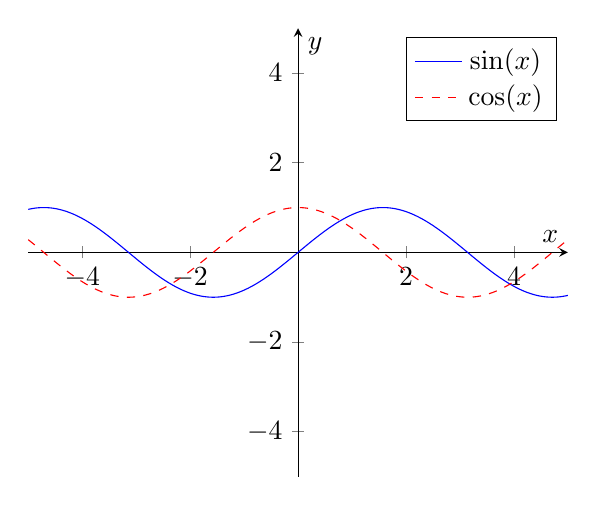
\begin{tikzpicture}
		\begin{axis}[
		xmin=-5, xmax=5, xlabel=$x$,
		ymin=-5, ymax=5, ylabel=$y$,
		samples=400,
		axis y line=middle,
		axis x line=middle,
		]
		\addplot+[mark=none] {sin(deg(x))};
		\addlegendentry{$\sin(x)$}
		\addplot+[mark=none, dashed] {cos(deg(x))};
		\addlegendentry{$\cos(x)$}
		\end{axis}
		\end{tikzpicture}
		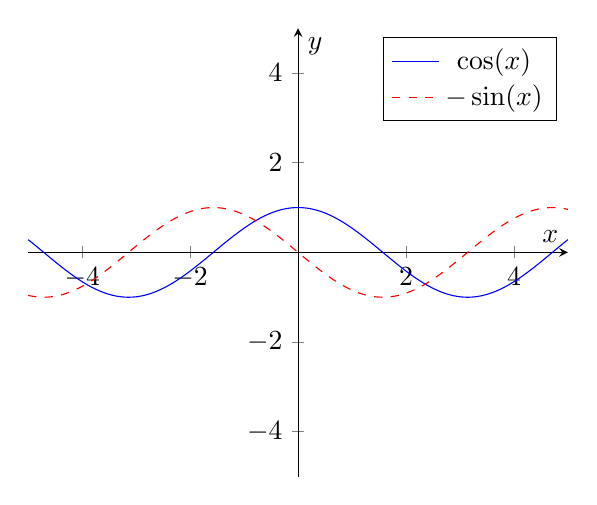
\begin{tikzpicture}
		\begin{axis}[
		xmin=-5, xmax=5, xlabel=$x$,
		ymin=-5, ymax=5, ylabel=$y$,
		samples=400,
		axis y line=middle,
		axis x line=middle,
		]
		\addplot+[mark=none] {cos(deg(x))};
		\addlegendentry{$\cos(x)$}
		\addplot+[mark=none, dashed] {- sin(deg(x))};
		\addlegendentry{$-\sin(x)$}
		\end{axis}
		\end{tikzpicture}\end{center}
\end{example}

\subsection{Rechenregeln}
\begin{*definition}
	Sei $f:D\subset K^n \to K^m$, $D$ offen.
	
	Falls $f$  \gls{diffbar} in allen $x_0\in D$, dann heißt $f$ \begriff{differenzierbar} auf $D$ und Funktion $f':D\to L(K^n, K^m)$ heißt \begriff{Ableitung} von $f$.
	
	Ist zusätzlich Funktion $f': D\to L(K^n, K^m)$ stetig, dann heißt Funktion $f$ \begriff{stetig differenzierbar} (auf $D$) bzw. \mathsymbol{C1}{$C^1$}\emph{-Funktion} (auf $D$).
	
	$C^1(D, K^m):= \left\lbrace f: D\to K^m \mid f \text{ stetig  \gls{diffbar} auf } D \right\rbrace$
\end{*definition}

\begin{example}
	\begin{enumerate}[label={\alph*)}]
		\item $f(x) = x^k\;\forall x\in\mathbb{R},\, k\in\mathbb{N}_{\ge 0}$ \\
		$\Rightarrow$ $f'(x) = k\cdot x^{k-1}\;\forall x\in \mathbb{R}$ \\
		$\Rightarrow$ offenbar stetige Funktion \\ $\Rightarrow$ $f\in C^1(\mathbb{R}, \mathbb{R})$
		
		\item $f(x) = e^x\;\forall x\in\mathbb{C}$ \\
		$\Rightarrow f'(x) = e^x \;\forall x\in\mathbb{C}$ stetig \\
		$\Rightarrow$ $f\in C^1(\mathbb{C},\mathbb{C})$
		
		\item $f(x) = \vert x \vert^2\;\forall x\in\mathbb{R}^n$ \\
		$\Rightarrow$ $f(x) = 2x\;\forall x\in\mathbb{R}^n$, offenbar stetig \\
		$\Rightarrow$ $f\in C^1(\mathbb{R}^n, \mathbb{R})$
	\end{enumerate}
\end{example}

\begin{example}
	\proplbl{ableitung_beipsiel_unstetige_ableitung}
	Sei $f:\mathbb{R}\to \mathbb{R}$ mit $f(0) = 0$, $f(x)=x^2\cdot \sin\left(\frac{1}{x}\right)$ $\forall x\neq 0$.
	
	\begin{center}\begin{tikzpicture}
		\begin{axis}[
		xmin=-5, xmax=5, xlabel=$x$,
		ymin=-5, ymax=5, ylabel=$y$,
		samples=400,
		axis y line=middle,
		axis x line=middle,
		]
		\addplot+[mark=none] {x^2*sin(deg(1/x))};
		\addlegendentry{$x^2\cdot \sin(\frac{1}{x})$}
		\end{axis}
		\end{tikzpicture}\end{center}
	
	Wegen \begin{align*}
		\frac{\vert x^2 \cdot \sin \frac{1}{x}\vert}{\vert x \vert} \le \vert x \vert \xrightarrow{x\neq 0} 0
	\end{align*}
	folgt{ \zeroAmsmathAlignVSpaces \begin{align*}
		& f(x) = o(\vert x \vert), x\to 0 \\
		\Rightarrow\;& f(x) = f(0) + 0\cdot (x - 0) + o(\vert x - 0\vert), x\to 0 \\
		\Rightarrow\;& f \text{  \gls{diffbar} in $x=0$ mit $f'(0) = 0$}
	\end{align*}}
	
	Rechenregeln liefern $x\neq 0$: \begin{align*}
		f'(x) = 2x\cdot\sin\frac{1}{x}- \cos\frac{1}{x} \quad\forall x\neq 0
	\end{align*}
	
	Für $x_k := \frac{1}{k\pi}$ gilt: \begin{align*}
		& \lim\limits_{k\to\infty} 2 x_k \cdot \sin \frac{1}{x_k} = 0,\; \lim\limits_{k\to\infty} \cos \frac{1}{x_k} = \pm 1 \\
		\Rightarrow\;& \lim\limits_{x\to 0} f'(x) \text{ existiert nicht} \\
		\Rightarrow\;& f\notin C^1(\mathbb{R}, \mathbb{R}),
	\end{align*}
	d.h. Ableitung einer stetigen Funktion muss \emph{nicht} stetig sein.
\end{example}

\begin{boldenvironment}[Man beobachtet]
	\hspace{0pt}
\begin{itemize}[topsep=-2pt]
	\item \propref{definition_ableitung} bzw. \propref{definition_ableitung_zwei_stern} sind häufig ungeeignet zum Bestimmen von $f'(x_0)$
	\item \propref{differentialquotient_prop} ist durchaus nützlich für konkrete Fälle im Fall $n=1$
	
	\emph{$\rightarrow$ Strategie:} Zurückführung auf einfachere Fälle durch Rechenregeln und Reduktion
\end{itemize}
\end{boldenvironment}

\begin{proposition}[Rechenregeln]
	\proplbl{ableitung_rechenregeln}
	Sei $D\in K^n$ offen, $f,g: D\to K^m$, $\lambda: D\to K$  \gls{diffbar} in $x_0\in D$ \\
	$\Rightarrow$ $(f\pm g): D\to K^m, (\lambda\cdot f):D\to K^m, (f\cdot g):D\to K$ sind  \gls{diffbar} in $x_0\in D$ und $\frac{1}{\lambda}:D\to K$ ist  \gls{diffbar} in $x_0$, falls $\lambda(x_0)\neq 0$
	mit
	\begin{enumerate}[label={\alph*)}]
		\item $(f\pm g)'(x_0) = f'(x_0) \pm g'(x_0)\in K^{m\times 1}$
		\item $(\lambda\cdot f)'(x_0) = \lambda (x_0)\cdot f'(x_0) + f(x_0)\cdot \lambda'(x_0)\in K^{m\times n}$
		\item $(f\cdot g)' (x_0) = \transpose{f(x_0)}\cdot g'(x_0) + \transpose{g(x_0)}\cdot f'(x_0)\in K^{m\times n}$
		\item $\left( \frac{1}{\lambda}\right)'(x_0) = - \frac{1}{\lambda(x_0)^2}\cdot \lambda'(x_0)\in K^{1\times n}$
	\end{enumerate}
\end{proposition}

\begin{conclusion}
	\proplbl{ableitung_quotientenregel}
	Seien $\lambda$, $\mu:D\to K$  \gls{diffbar} in $x_0$, $D$ offen und $\lambda(x_0)\neq 0$ \\
	$\Rightarrow$ $\left( \frac{\mu}{\lambda} \right): D\to K$  \gls{diffbar} in $x_0$ mit \begin{align*}
		\left( \frac{\mu}{\lambda} \right)' (x_0) = \frac{\lambda(x_0)\cdot \mu'(x_0) - \mu(x_0) \cdot \lambda'(x_0)}{\lambda(x_0)^2}\in K^{1\times n}
	\end{align*}
\end{conclusion}

\begin{proof}[\propref{ableitung_quotientenregel}]
	Setzte in \propref{ableitung_rechenregeln} $f=\mu$ (d.h. $m=1$) und betr. Produkt $\frac{1}{\lambda}\cdot \mu$.
\end{proof}

\begin{proof}[\propref{ableitung_rechenregeln}]
	Nach \propref{definition_ableitung_proposition} c) existieren $P,Q: D\to L(K^n, K^m)$, $\Lambda:D\to L(K^n, K)$ mit
\begin{itemize}[topsep=\dimexpr -\baselineskip / 3\relax]
	\item $f(x) = f(x_0) + P(x) \cdot (x - x_0)$, $\lim\limits_{x\to x_0} P(x) = f'(x_0)$
	\item $g(x) = g(x_0) + Q(x) \cdot (x - x_0)$, $\lim\limits_{x\to x_0} Q(x) = g'(x_0)$
	\item $\lambda(x) = \lambda(x_0) + \Lambda(x_0) \cdot (x - x_0)$, $\lim\limits_{x\to x_0} \Lambda(x) = \lambda'(x_0)$
\end{itemize}
und mit \propref{definition_ableitung_proposition} c) ergibt sich die Behauptung wie folgt:
\begin{enumerate}[label={\alph*)}]
	\item $f(x) + g(x) = f(x_0) + g(x_0) + \underbrace{\big( P(x) + Q(x) \big)}_{\mathclap{x\to x_0:\; f'(x_0) + g'(x_0)\in L(K^n, K^m)}}\cdot (x - x_0)$ \\
	$\Rightarrow$ Behauptung
	\item $\lambda(x)\cdot f(x) = \lambda(x_0) \cdot f(x_0) + \underbrace{\left[ \lambda(x_0) \cdot P(x) + \underbrace{f(x_0)\cdot \Lambda(x)}_{\in K^{m\times n}} + \underbrace{\Lambda(x_) \cdot (x - x_0)}_{\in K} \cdot P(x) \right]}_{\xrightarrow{x\to x_0}\lambda(x_0)\cdot f'(x_0) + f(x_0)\cdot \lambda'(x_0)\in L(K^m, K^n)} \cdot (x - x_0)$ \\
	$\Rightarrow$ Behauptung
	\item analog zu b)
	\item $\frac{1}{\lambda(x)} = \frac{1}{\lambda(x_0)} - \frac{\lambda(x) - \lambda(x_0)}{\lambda(x_0)\cdot \lambda(x)} = \frac{1}{\lambda(x_0)} + \underbrace{\left( - \frac{1}{\lambda(x_0)\cdot\lambda(x)}\cdot \Lambda(x)\right)}_{\mathclap{\xrightarrow{x\to x_0}-\frac{1}{\lambda(x_0)^2}\cdot \lambda'(x_0)\in L(K^n, K)}} (x - x_0)$\\
	$\Rightarrow$ Behauptung
\end{enumerate}
\end{proof}

\begin{example}
	Sei $f:D\in K^n\to K^m$, $c\in K$, $f$  \gls{diffbar} in $x_0\in D$\\
	$\xRightarrow{\ref{ableitung_rechenregeln}\ b)} (c\cdot f) = c\cdot f'(x_0)$ (da $c$ konst. Funktion $D\to K$)
\end{example}

\begin{example}[Polynom]
	Sei $f:K\to K$, Polynom $f(x) = \sum\limits_{l=0}^{k}a_l x^l$ \\
	$\Rightarrow$ $f$  \gls{diffbar} $\forall x_0\in K$ mit $f'(x_0) = \sum\limits_{l=1}^k l a_l x_0^{l-1}$
\end{example}

\begin{example}
	Sei $f=\frac{f_1}{f_2}$ rationale Funktion auf $\mathbb{R}$ (d.h. $f_1, f_2:K\to K$ Polynom) \\
	$\Rightarrow$ $f$ ist  \gls{diffbar} auf $K\setminus \{ \text{Nullstellen von }f_2 \}$
\end{example}

\begin{example}[Tangens und Cotangens]
	\proplbl{ableitung_beispiel_tangens}
	$\tan: K\setminus \{ \frac{\pi}{2} + k\cdot \pi \mid k\in\mathbb{Z} \}\to K$, $\cot:K\setminus \{ k\cdot \pi \mid k\in\mathbb{Z} \} \to K$ \\[\dimexpr - \baselineskip / 2 \relax]
	\zeroAmsmathAlignVSpaces \begin{alignat*}{3}
	\xRightarrow{\text{Quotientenregel}}&\;\;& \tan'(x_0)&= \frac{\sin'(x_0)\cos (x_0) - \cos (x_0) \cdot \sin(x_0)}{\left( \cos(x_0)\right)^2} &&\\
	&& &= \frac{\cos^2(x_0) + \sin^2(x_0)}{\cos^2(x_0)} = \frac{1}{\cos^2(x_0)} && \forall x_0\in \text{ Definitionsbereich} \\
	&& \cot'(x_0) &= - \frac{1}{\sin^2(x_0)}&&\forall x_0\in\text{ Definitionsbereich}
	\end{alignat*}
	\begin{center}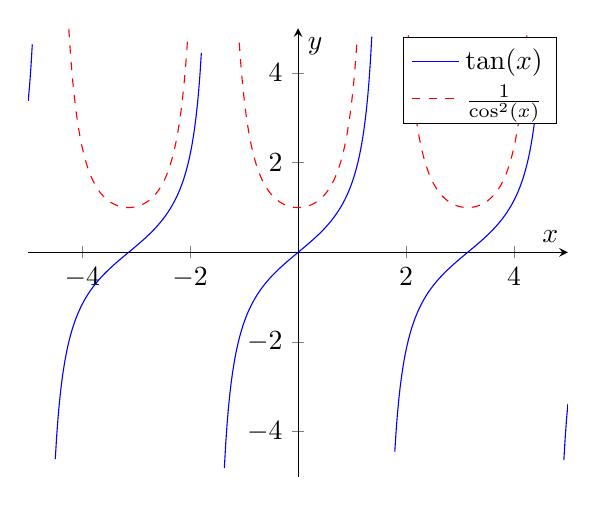
\begin{tikzpicture}
		\begin{axis}[
		xmin=-5, xmax=5, xlabel=$x$,
		ymin=-5, ymax=5, ylabel=$y$,
		samples=400,
		axis y line=middle,
		axis x line=middle,
		restrict y to domain=-5:5
		]
		\addplot+[mark=none] {tan(deg(x))};
		\addlegendentry{$\tan(x)$}
		\addplot+[mark=none, dashed] {1/(cos(deg(x)))^2};
		\addlegendentry{$\frac{1}{\cos^2(x)}$}
		\end{axis}
		\end{tikzpicture}
		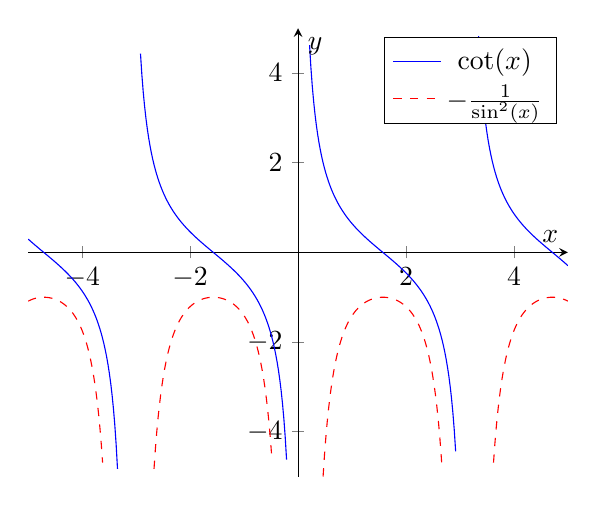
\begin{tikzpicture}
		\begin{axis}[
		xmin=-5, xmax=5, xlabel=$x$,
		ymin=-5, ymax=5, ylabel=$y$,
		samples=400,
		axis y line=middle,
		axis x line=middle,
		restrict y to domain=-5:5
		]
		\addplot+[mark=none] {cot(deg(x))};
		\addlegendentry{$\cot(x)$}
		\addplot+[mark=none, dashed] {-1/(sin(deg(x))^2)};
		\addlegendentry{$-\frac{1}{\sin^2(x)}$}
		\end{axis}
		\end{tikzpicture}\end{center}
\end{example}

\begin{proposition}[Kettenregel]
	\proplbl{ableitung_kettenregel}
	Sei $f:D\subset K^n\to K^m$, $g:\tilde{D}\subset K^m\to K^l$, $D$,$\tilde{D}$ offen, $f$  \gls{diffbar} in $x_0\in D$, $g$  \gls{diffbar} in $f(x_0)\in\tilde{D}$ \\
	$\Rightarrow$ $g\circ f: D\to K^l$  \gls{diffbar} in $x_0$ mit $(g\circ f)' = g'(f(x))\cdot f'(x)$ ($\in K^{l\times n}$)
\end{proposition}

\begin{proof}
	Nach \propref{definition_ableitung_proposition} c) exisitert $P:D\to L(K^n, K^m)$, $Q:\tilde{D}\to K(K^m, K^l)$ mit
	\zeroAmsmathAlignVSpaces**
	\begin{alignat}{2}
	\proplbl{ableitung_kettenregel_beweis_f} && f(x) &= f(x_0) + P(x)(x - x_0), \lim\limits_{x\to x_0} P(x) = f'(x_0) \\
	\proplbl{ableitung_kettenregel_beweis_g} && g(y) &= g(f(x_0)) + Q(y)(y - f(x_0)), \lim\limits_{y\to f(x_0)} Q(y) = g'(f(x_0)) \\
	\notag \Rightarrow\quad && (g\circ f)(x) &= g(f(x)) \overset{\eqref{ableitung_kettenregel_beweis_g}}{=} g(f(x_0)) + Q(f(x)(f(x) - f(x_0)) \\
	\notag&& &= (g\circ f)(x_0) + \underbrace{\left[ Q(f(x)) \cdot P(x)\right]}_{\mathclap{\xrightarrow{x\to x_0}g'(f(x_0))\cdot f'(x_0)}} (x - x_0)
	\end{alignat}
	$\xRightarrow{\ref{definition_ableitung_proposition}\,c)}$ Behauptung
\end{proof}

\begin{example}[$x$ im Exponenten]
	\proplbl{ableitung_beispiel_exponentialfunktion}
	Sei $f:\mathbb{R}\to \mathbb{R}$, $f(x) = a^x$ ($a\in\mathbb{R}_{\ge 0}$, $a\neq 1$).
	
	Offenbar $a^x = \left(e^{\ln a}\right)^x = e^{x\cdot \ln a}$\\
	$\Rightarrow$ $f(x) = g(h(x))$ mit $g(y) = e^y$, $h(x) = x\cdot \ln a$
	
	Wegen $g'(y) = e^y$ $\forall y\in\mathbb{R}$, $h'(x) = \ln a$ $\forall x\in K$ \\[\dimexpr -\baselineskip / 2 \relax]
	\zeroAmsmathAlignVSpaces \begin{alignat*}{2}
	\xRightarrow{\text{\propref{ableitung_kettenregel}}}\quad&& f'(x_0) &= g'(x_0\cdot \ln a)\cdot f'(x_0) = e^{x_0\cdot \ln a}\cdot \ln a = a^x\cdot \ln a \quad\forall x_0\in\mathbb{R}
	\end{alignat*}
	\begin{center}\begin{tikzpicture}
		\begin{axis}[
		xmin=-5, xmax=5, xlabel=$x$,
		ymin=-5, ymax=5, ylabel=$y$,
		samples=400,
		axis y line=middle,
		axis x line=middle,
		]
		\addplot+[mark=none] {2^x};
		\addlegendentry{$2^x$}
		\addplot+[mark=none, dashed] {2^x*ln(2)};
		\addlegendentry{$2^x\cdot \ln(2)$}
		\end{axis}
		\end{tikzpicture}\end{center}
\end{example}

\begin{example}[Logarithmus]
	\proplbl{ableitung_beispiel_logarithmus}
	Sei $f:\mathbb{R}_{>0} \to \mathbb{R}$, $f(x) = \log_a x$ ($a\in\mathbb{R}_{>0}\setminus\{1\}$)
	
	Fixiere $x_0\in \mathbb{R}_{>0}$, sei $\{x_n\}$ beliebige Folge in $\mathbb{R}_{>0}$ mit $x_n\to x_0$
	\zeroAmsmathAlignVSpaces*[5pt] \begin{alignat*}{1}
		\xRightarrow{\text{$f$ stetig}}\;& y:= \log_a x_n \to \log_a x_0 =: y_0 \\
		\Rightarrow\;\;&\!\! \lim\limits_{n\to \infty} \frac{f(x_n) - f(x_0)}{x_n - x_0} = \lim\limits_{n\to \infty} \frac{\log_a(x_n) - \log_a(x_0)}{a^{\log_a(x_n)} - a^{\log_a(x_0)}} = \lim\limits_{n\to \infty} \dfrac{1}{\frac{a^{y_n} - a^{y_0}}{y_n - y_0}} \overset{\ref{ableitung_beispiel_exponentialfunktion}}{=}{\frac{1}{a^{y_0}\cdot \ln(a)}} \\
		\xRightarrow{\{x_n\}\text{ bel.}}\;& f'(x_0) = \frac{1}{x_0\cdot \ln a}\quad\forall x>0
	\end{alignat*}
	
	Spezialfall: $(\ln(x))' = \frac{1}{x}$ $\forall x>0$
	\begin{center}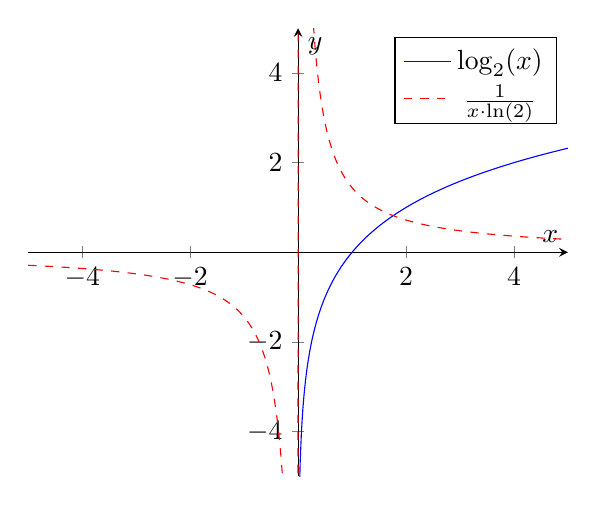
\begin{tikzpicture}
		\begin{axis}[
		xmin=-5, xmax=5, xlabel=$x$,
		ymin=-5, ymax=5, ylabel=$y$,
		samples=400,
		axis y line=middle,
		axis x line=middle,
		]
		\addplot+[mark=none] {log2(x)};
		\addlegendentry{$\log_2(x)$}
		\addplot+[mark=none, dashed] {1/(x*ln(2))};
		\addlegendentry{$\frac{1}{x\cdot\ln(2)}$}
		\end{axis}
		\end{tikzpicture}\end{center}
\end{example}

\begin{example}
	Sei $f:\mathbb{R}_{>0}\to \mathbb{R}$, $f(x) = x^r$ ($r\in\mathbb{R}$)
	
	Wegen $x^r = e^{r\cdot \ln x}$ liefert Kettenregeln (analog zu \propref{ableitung_beispiel_exponentialfunktion}) \begin{align*}
		f'(x_0) = \frac{r\cdot e^{r\cdot \ln x_0}}{x_0} = \frac{r\cdot x_0^r}{x_0} = r\cdot x_0^{r - 1} \quad\forall x_0>0
	\end{align*}
	
	Spezialfall: $f(x) = \frac{1}{x^k}$ $\Rightarrow$ $f'(x) = - \frac{k}{x^{k+1}}$
	
	Zu \propref{ableitung_beipsiel_unstetige_ableitung}:\begin{align*}
		f'(x) = 2x\cdot \sin\frac{1}{x} + x^2\cdot \cos\frac{1}{x} \cdot \left( - \frac{1}{x^2}\right) = 2x\cdot \sin\frac{1}{x} - \cos\frac{1}{x}
	\end{align*}
\end{example}

\begin{proposition}[Reduktion auf skalare Funktionen]
	\proplbl{ableitung_proposition_reduktion}
	Sei $f=(f_1, \dotsc, f_m): D\subset K^n\to K^m$, $D$ offen, $x_0\in D$. Dann gilt:\begin{center}
		$f$  \gls{diffbar} in $x_0$ $\Leftrightarrow$ alle $f_j$  \gls{diffbar} in $x_0$ $\forall j=1,\dotsc,m$
	\end{center}

	Im Fall der Differenzierbarkeit hat man: \begin{align}
		\proplbl{ableitung_jacobimatrix}
		f'(x_0) = \begin{pmatrix}
			f_1'(x_0) \\
			\vdots \\
			f_m'(x_0)
		\end{pmatrix} \in K^{m\times n}
	\end{align}
\end{proposition}
\smiley{} Wenn Sie das nächste mal aus der Disko kommen, zuviel getrunken haben und den Namen 
ihrer Freundin nicht mehr kennen, sollten sie sich daran aber noch erinnern: \smiley{} \\

\begin{remark}
	Mit \propref{ableitung_proposition_reduktion} kann man die Berechnungen der Ableitungen stets auf skalare Funktionen $f:D\subset K^n\to K$ zurückführen. Die Matrix in \propref{ableitung_jacobimatrix} besteht aus $m$ Zeilen $f_j'(x_0)\in K^{1\times m}$.
\end{remark}

\begin{example}
	Sei $f:\mathbb{R}\to \mathbb{R}^2$ mit \begin{align*}
		f(t) &= \begin{pmatrix}
			t\cdot \cos( 2\pi t) \\ t\cdot \sin(2\pi t)
		\end{pmatrix}, & f'(t) &= \begin{pmatrix}
			\cos(2\pi t) - t\cdot \sin(2\pi t)\cdot 2\pi \\ \sin(2\pi t)+ t\cdot\cos(2\pi t)\cdot 2\pi
		\end{pmatrix} \in \mathbb{R}^{2\times 1},
	\end{align*}
	und $f'(0) = \binom{1}{0}$, $f'(1) = \binom{1}{2\pi}$.
\end{example}

\begin{lemma}
	\proplbl{ableitung_spezialfall_reduktion_proposition}
	Sei $f=(f_1, f_2):D\subset K^n\to K^k\times K^l$, $D$ offen, $x_0\in D$.
	
	Funktion $f$ ist  \gls{diffbar} in $x_0$ genau dann, wenn $f_1:D\to K^k$ und $f_2 :D\to K^l$  \gls{diffbar} in $x_0$.
	
	Im Falle der Differenzierbarkeit gilt\begin{align}
		\proplbl{ableitung_spezialfall_reduktion}
		f'(x_0) = \begin{pmatrix}
			f_1'(x_0) \\ f_2'(x_0)
		\end{pmatrix} \in K^{(k+l)\times n}
	\end{align}
	
	\begin{hint}
		Da $K^k\times K^l$ mit $K^{k+l}$ identifiziert werden kann, kann man $f$ auch als Abbildung von $D$ nach $K^{k+l}$ ansehen. Dementsprechend kann die Matrix in \propref{ableitung_spezialfall_reduktion} der Form \begin{align*}
			\begin{pmatrix}
				(k\times n) \text{ Matrix} \\
				(l\times n) \text{ Matrix}
			\end{pmatrix}
		\end{align*}
		auch als $((k+l)\times n)$-Matrix aufgefasst werden.
	\end{hint}
\end{lemma}

\begin{proof}\hspace*{0pt}
	\NoEndMark
	\begin{itemize}[topsep=\dimexpr - \baselineskip / 3\relax]
		\item["`$\Rightarrow$"'] Man hat
		\zeroAmsmathAlignVSpaces[3pt][3pt]
		\begin{alignat}{2}
				\proplbl{ableitung_beweis_lemma_spezialfall_reduktion} && f(x) &= f(x_0) + f'(x_0)\cdot(x - x_0) + R(x)\cdot (x - x_0), \, \;R(x) \xrightarrow{x\to x_0}0
			\intertext{da $f'(x_0)$, $R(x)\in L(K^n, K^k\times K^l)$}
				\notag\Rightarrow&\;\;& f'(x_0) &= (A_1, A_2), \; R(x) = \big( R_1(x), R_2(x) \big))
			\intertext{mit $A_1, R_1(x)\in L(K^n, K^k)$, $A_2, R(x)\in L(K^n, K^l)$}
				\proplbl{ableitung_beweis_lemma_spezialfall_reduktion_einzelableitung} \xRightarrow{\eqref{ableitung_beweis_lemma_spezialfall_reduktion}}&& f_j(x)&= f_j(x_0) + A_j \cdot (x - x_0) + R_j(x) (x - x_0),\;R_j(x)\xrightarrow{x\to x_0}0 \\
				\notag\Rightarrow&& f_j & \text{ ist  \gls{diffbar} in $x_0$ mit $f_j'(x_0) = A_j$, $j=1,2$}
		\end{alignat}
		$\Rightarrow$ Behauptung
		\item["`$\Leftarrow$"'] (es gilt auch \eqref{ableitung_beweis_lemma_spezialfall_reduktion_einzelableitung} mit $A_j = f_j'(x_0)$)
		
		Setzte \begin{align*}
		 &A=\begin{pmatrix}
			f_1'(x) \\ f_2'(x)
		\end{pmatrix},\; R(x) = \begin{pmatrix}
			R_1(x) \\ R_2(x)
		\end{pmatrix} \\
		\xRightarrow{\eqref{ableitung_beweis_lemma_spezialfall_reduktion_einzelableitung}}\;& A, R(x)\in L(K^n, K^k\times K^l) \\
		\xRightarrow{\text{mit }A_j=f_j'(x_0)}\; & f(x)= f(x_0) + A(x - x_0) + R(x)(x - x_0), R(x)\xrightarrow{x\to x_0}0
		\end{align*}
		$\Rightarrow$ $f$  \gls{diffbar} in $x_0$ und \eqref{ableitung_spezialfall_reduktion} gilt.\hfill\csname\InTheoType Symbol\endcsname
	\end{itemize}
\end{proof}

\begin{proof}[\propref{ableitung_proposition_reduktion}]
	Mehrfache Anwendung von \propref{ableitung_spezialfall_reduktion_proposition} (z.B. mit $k=1, l = m - j$ für $j=1,\dotsc, m-1$)
\end{proof}